\documentclass[landscape, 11pt]{report}

% Packages
\usepackage[landscape]{geometry}
\usepackage{amsmath}
\usepackage{xcolor}
\usepackage[utf8]{inputenc}
\usepackage[russian]{babel}
\usepackage{geometry}
\usepackage{graphicx}

% Options
\graphicspath{ {../figures/} {./figures/}}
\geometry{left=2.5cm,right=2.5cm,top=2.5cm,bottom=2.5cm}
\setlength\parindent{0pt}

% Title
\title{
	
\includegraphics[scale=0.07]{logo}\\
	\vspace{0.5em}
	Языки программирования. Семантика и система типов\\
	\vspace{0.2em}
	\Large Теоретическое задание. Тема 14
}
\author{Бронников Егор}
\date{}


\begin{document}
	
	% Титул
	
	\maketitle
	
	\vspace{-0.5cm}
	\hrule
	\vspace{0.5cm}
	
	% Задание 1
	
	\textbf{Задание 1.} Предположите кодировку для типов-сумм в Cистеме F$_{<:}$ (аналогично кодировке пар):
	
	\begin{itemize}
		\item[] (a) определите тип $Sum \; T_1 \; T_2$;
		\item[] (b) выпишите типы и определения \textit{функций} $left$, $right$, $match$, соответствующих синтаксическим конструкциям $inl(t)$, $inr(t)$ и $case \; t \; of \; inl(x_1) \Rightarrow t_1 \; | \; inr(x_2) \Rightarrow t_2$;
		\item[] (c) покажите (построив соответствующее дерево вывода), что выполняется следующие правило:
		\begin{center}
			$\dfrac{\Gamma \vdash S_1 <: T_1 \quad \Gamma \vdash S_2 <: T_2}{\Gamma \vdash Sum \; S_1 \; S_2 \; <: \; Sum \; T_1 \; T_2}$ S-Sum
		\end{center}
	\end{itemize}
	
	\vspace{0.2cm}
	
	\textit{Решение.}
	
	\vspace{0.2cm}
	
	\textit{(a) Определение типа $Sum \; T_1 \; T_2$.}
	
	\vspace{0.2cm}
	
	$Sum \; T_1 \; T_2 = \forall X . (T_1 \rightarrow X) \rightarrow (T_2 \rightarrow X) \rightarrow X$
	
	\vspace{0.2cm}
	
	\textit{(b) Типы и определения \textit{функций} $left$, $right$, $match$, соответствующих синтаксическим конструкциям $inl(t)$, $inr(t)$ и \newline $case \; t \; of \; inl(x_1) \Rightarrow t_1 \; | \; inr(x_2) \Rightarrow t_2$.}
	
	\vspace{0.2cm}
	
	$left = \Lambda X. \Lambda T_1. \Lambda T_2. \lambda r: T_1. \lambda f_1 : T_1 \rightarrow X . \lambda f_2 : T_2 \rightarrow X . f_1 \, r \; as \; Sum \, T_1 \, T_2$
	
	$right = \Lambda X. \Lambda T_1. \Lambda T_2. \lambda r: T_2. \lambda f_1 : T_1 \rightarrow X . \lambda f_2 : T_2 \rightarrow X . f_2 \, r \; as \; Sum \, T_1 \, T_2$
	
	$match = \Lambda X . \Lambda T_1 . \Lambda T_2. \lambda r : Sum \, T_1 \, T_2 . \lambda y_1 : T_1 \rightarrow X . \lambda y_2 : T_2 \rightarrow X . r \, [X] \; y_1 \; y_2$
	
	\vspace{0.25cm}
	
	\textit{(c) Дерево вывода.}
	
	\begin{center}
		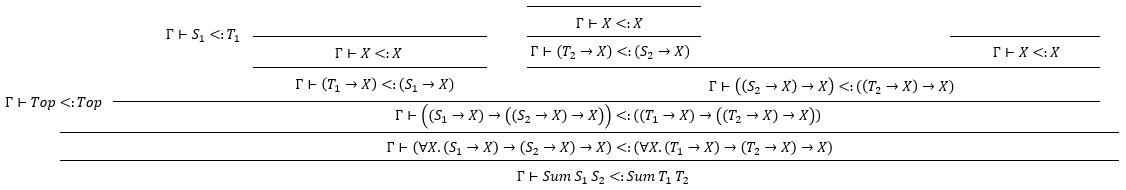
\includegraphics[scale=0.7]{solution}
	\end{center}

	\hrule
	
	\newpage
	
	% Задание 2
	
	\hrule
	\vspace{0.5cm}

	\textbf{Задание 2.} Для каждого из следующих типов ядерной Системы F$_{<:}$, постройте (любой) терм этого типа вместе с соответствующим деревом вывода типа (включая поддеревья вывода подтипизации, где необходимо) или покажите, что это невозможно:
	
	\begin{itemize}
		\item[] (a) $\forall X <: Top. \; \forall Y <: X . X \rightarrow Y$
		\item[] (b) $\forall X <: Top. \; \forall Y <: X . Y \rightarrow X$
		\item[] (c) $\forall X <: Top. \; \forall Y <: X . Y \; \forall Z <: Y. Y \rightarrow (X \rightarrow Z) \rightarrow Z$
	\end{itemize}
	
	\textit{Решение.}
	
	\vspace{0.2cm}
	
	\textit{(a) $\forall X <: Top. \; \forall Y <: X . X \rightarrow Y$}
	
	\vspace{0.2cm}
	
	\textit{Ответ.} Невозможно построить терм, так как нет гарантий, что любой элемент типа $X$ можно преобразовать в любой элемент типа $Y$, потому что $Y$ может быть любым подтипом $X$, включая пустой тип.
	
	\vspace{0.2cm}
	
	\textit{(b) $\forall X <: Top. \; \forall Y <: X . Y \rightarrow X$}
	
	\vspace{0.2cm}
	
	\textit{Ответ.} $-$

	\vspace{0.2cm}

	\textit{(c) $\forall X <: Top. \; \forall Y <: X . Y \; \forall Z <: Y. Y \rightarrow (X \rightarrow Z) \rightarrow Z$}

	\vspace{0.2cm}

	\textit{Ответ.} $-$

	\vspace{0.5cm}
	\hrule
	\vspace{0.5cm}

	% Задание 3
	
	\textbf{Задание 3.} Постройте дерево вывода, соответствующее алгоритму проверки типов для ядра $F_{<:}$ для соответствующих замкнутых термов:
	
	\begin{itemize}
		\item[] (a) $(\lambda X <: Top. \, \lambda x : X . \, x ) \, [\{a : Nat, b : Bool \}] \, \{a = 0, b = true, c = false\} : 
		\{a : Nat\} $
		\item[] (b) $\lambda X <: Top . \, \lambda Y <: X \rightarrow X . \, \lambda Z <: X \rightarrow Y . \, \lambda f : Z . \, \lambda x : X . \, f \; x \; x : \forall X <: Top . \, \forall Y <: X \rightarrow X . \,\forall Z <: X \rightarrow Y . \, Z \rightarrow X \rightarrow X$
		\item[] (c) $\forall X <: Top . \, \lambda f : (\forall Y <: X \rightarrow X . \, Y) . \, \lambda x : X . \, f \; x : \forall X <: \{a : Nat\} . \, (\forall Y <: X \rightarrow \{a : Nat\} . \, X \rightarrow X) \rightarrow X \rightarrow \{a : Nat\}$
	\end{itemize}
	
	\vspace{0.2cm}
	
	\textit{Решение.}
	
	\begin{center}
		$-$
	\end{center}
	
	\hrule

\end{document}
